\documentclass[11pt,a4paper]{article}
\usepackage{paperstyle}
\usepackage{graphicx}
\graphicspath{{../figures/}}

\title{Depositing More Should Not Earn Less}
\researchsubtitle{Supplier income monotonicity and rate curve design in pooled lending markets}
\researchshorttitle{Depositing More Should Not Earn Less}
\author{%
\begin{tabular}{c@{\hspace{3em}}c}
Ahzam Khan & Cavey Cool \\
\small\href{mailto:ahzam.main@gmail.com}{ahzam.main@gmail.com} &
\small\href{mailto:caveycool@gmail.com}{caveycool@gmail.com}
\end{tabular}}
\date{September 2026}
\hypersetup{pdftitle={Depositing More Should Not Earn Less},pdfauthor={Ahzam Khan and Cavey Cool},pdfsubject={Supplier income monotonicity and rate curve design in pooled lending markets}}

\begin{document}
\maketitle

\begin{abstract}
Utilization dependent interest rate models can create a counterintuitive supplier incentive: adding liquidity may reduce a supplier's total interest income even as the supplier's balance increases. A supplier holding a fraction $\alpha$ of final pool supply keeps income nondecreasing with a marginal deposit exactly when $\alpha(1+\eta)\leq1$, where $\eta$ is the elasticity of the borrow rate with respect to utilization. When the condition fails, the supplier can instead raise its income by withdrawing, which pushes utilization further up. A protocol turns this into a design constraint by choosing a protection profile $\bar\alpha(U)$, the largest supplier share it intends to protect. That choice induces an elasticity envelope $E(U)=(1-\bar\alpha(U))/\bar\alpha(U)$, and integrating the envelope describes every admissible curve. A flat target gives a constant ceiling and a power law boundary; protecting every fresh depositor gives the profile $1-U$ and a hyperbolic boundary. Neither guarantee implies the other, and imposing both takes the smaller of their envelopes. We give piecewise linear and analytic constructions and compare them on a multiple kink USDT market whose parameters are drawn from a deployed configuration. The constraint does not determine the level of interest income: a compliant floor can reduce earnings, while a repair that only raises rates preserves supplier income under the same market history at a cost to borrowers. Fixed knots introduce restrictions beyond the continuous endpoint bound. As an extension, requiring a continuous derivative makes the minimum worst case elasticity $K^*$ unattainable rather than merely minimal.
\end{abstract}

\section{Introduction}

Pooled lending protocols commonly determine interest rates as a function of utilization. A standard design increases the borrow rate gradually below an optimal utilization level and much more aggressively above it. The steep branch improves incentives to restore liquidity under stress, but it also creates a supplier price impact problem: an additional deposit lowers utilization, which lowers the borrow rate, and the lower rate applies to the supplier's entire balance.

Consequently, a supplier may be better off withholding capital, or withdrawing it. This is not hypothetical: on a lending market at high utilization, one of us found that the profitable action was to deposit less than the balance held, which is the state in which the pool can least afford it.

The role of this paper is to give an exact condition under which this cannot happen, to describe the rate curves that satisfy it, and to separate what such a guarantee promises from what it costs. The rest of the paper proceeds as follows. In Section~\ref{sec:failure} we work the failure through in numbers. In Sections~\ref{sec:model}--\ref{sec:family} we derive the income condition and the admissible family of rate curves it induces. In Sections~\ref{sec:fixed} and \ref{sec:fresh} we develop two protection guarantees and show that both are instances of the same construction, and in Section~\ref{sec:minimal} we give a power law repair. In Sections~\ref{sec:multi} and \ref{sec:earnings} we take a market with several kinks and separate protection from pricing. Lastly, in Section~\ref{sec:onchain} we state the check a protocol would implement. Detailed constructions, sensitivity studies and the smooth extension are collected in the appendices.

\section{The Failure Mode}
\label{sec:failure}

Consider a market with optimal utilization $O=80\%$, a borrow rate of $R_o=5\%$ at that point, and a maximum borrow rate of $R_{\max}=100\%$ at full utilization, connected by straight lines. This is a standard kinked curve; the jump above the kink is large but not unusual.

Let the market hold \$10 million of supply against \$8.3 million of borrowings, so utilization is $83\%$. The market is above its own optimal level, which is precisely the state in which the protocol wants more supply, and a supplier holding \$1 million of the pool provides it. That supplier earns about \$159{,}800 a year before the deposit, and after adding \$375{,}000, which is exactly enough to return the market to optimal utilization, earns about \$55{,}000. The balance has grown by $37.5\%$ and the income has fallen by $66\%$. Depositing past the kink recovers only part of the loss, and as Figure~\ref{fig:failure-mode} shows, the income never returns to where it started. The same supplier does better by going the other way: withdrawing about \$302{,}000 raises its income to about \$188{,}300, $18\%$ more on $30\%$ less capital, and moves utilization from $83\%$ to about $85.6\%$, further from the level the protocol is trying to restore.

\begin{figure}[htbp]
\centering
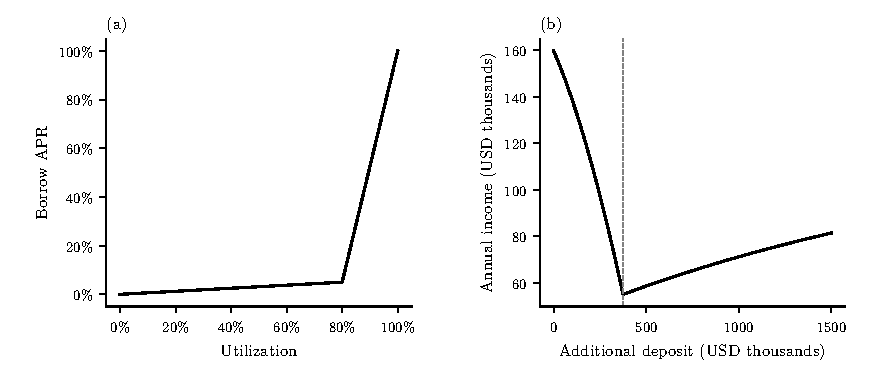
\includegraphics[width=\textwidth]{T01-failure.pdf}
\caption{(a) The illustrative kinked borrow rate. (b) Annualized income of a supplier initially holding $10\%$ of a \$10 million pool, with \$8.3 million of fixed borrowing, against the change in its balance; negative values are withdrawals. The dashed line marks the deposit that returns utilization to $80\%$, and the dot marks the income-maximizing withdrawal.}
\label{fig:failure-mode}
\end{figure}

Two things about this example are worth keeping in mind. The loss is not caused by the deposit being large but by the rate being sensitive, and the worst point is the kink itself rather than full utilization. Both follow from the condition derived below, and neither is visible from the slope of the curve alone.

\section{Model}
\label{sec:model}

Let
\begin{itemize}
  \item $T$ denote total supplied tokens after the supplier's transaction,
  \item $B$ denote total borrowings,
  \item $b$ denote the supplier's resulting deposited balance,
  \item $U=B/T$ denote utilization,
  \item $R_b(U)$ denote the borrow rate at utilization $U$, and
  \item $R_s(U)$ denote the supply rate.
\end{itemize}

We assume the rate is nondecreasing, continuous and piecewise continuously differentiable, with $R_b(U)>0$ for $U>0$. Corners are allowed. The formulas below apply inside each smooth segment; at a corner an additional deposit enters from the side of lower utilization. A zero base rate at $U=0$ is permitted unless a later guarantee rules it out.

Ignoring fees, aggregate borrowers pay $BR_b(U)$ in annualized interest. Distributed across $T$ supplied tokens, the supply rate is therefore
\[
R_s(U)=\frac{BR_b(U)}{T}=UR_b(U)
\]
and the supplier's annualized interest income is
\[
I=bR_s(U)=bUR_b(U)
\]
Write the supplier's share of final pool supply as
\[
\alpha=\frac{b}{T}
\]
Measuring $\alpha$ after the transaction rather than before it is deliberate, since the monotonicity condition applies to the supplier's resulting state once the marginal deposit has been added.

Consider an infinitesimal increase $d\delta$ in the same supplier's deposit, holding $B$ fixed during the transaction. Then $db/d\delta=1$ and $dT/d\delta=1$, so
\[
\frac{dU}{d\delta}
=\frac{d}{d\delta}\left(\frac{B}{T}\right)
=-\frac{B}{T^2}
=-\frac{U}{T}
\]
and additional supply reduces utilization locally. A constant fraction $f<1$ withheld from borrower interest multiplies supplier income and its derivative by $1-f$, leaving the sign condition unchanged. A utilization dependent fee would need to be included in the derivative. Income here is an annualized flow at a state, not interest already earned over time.

\section{Supplier Income Monotonicity}
\label{sec:condition}

Differentiating $I=bUR_b(U)$ with respect to the additional deposit gives
\[
\begin{aligned}
\frac{dI}{d\delta}
&=\frac{d}{d\delta}\left[bUR_b(U)\right] \\
&=UR_b(U)+b\left[R_b(U)+UR_b'(U)\right]\frac{dU}{d\delta} \\
&=UR_b(U)-\frac{bU}{T}\left[R_b(U)+UR_b'(U)\right] \\
&=UR_b(U)\left[1-\frac{b}{T}\left(1+\frac{UR_b'(U)}{R_b(U)}\right)\right]
\end{aligned}
\]

\begin{proposition}[Marginal supplier income]
For a marginal deposit made while borrowings are fixed,
\[
\boxed{
\frac{dI}{d\delta}
=UR_b(U)\left[1-\alpha\left(1+\frac{UR_b'(U)}{R_b(U)}\right)\right]
}
\]
\end{proposition}

Two competing effects sit inside that bracket: the marginal dollar earns the current supply rate $UR_b(U)$, while the fall in utilization it causes lowers the rate applied to everything the supplier already holds. The size of the second effect is measured by $UR_b'(U)/R_b(U)$, the elasticity of the borrow rate with respect to utilization,
\[
\boxed{
\eta(U)=\frac{U}{R_b(U)}\frac{dR_b}{dU}
=\frac{UR_b'(U)}{R_b(U)}
=\frac{d\ln R_b}{d\ln U}
}
\]
The logarithmic form on the right is what Section~\ref{sec:family} works with. Substituting it into the income derivative gives the identity this paper is built on,
\[
\boxed{
\frac{dI}{d\delta}
=UR_b(U)\left[1-\alpha(1+\eta(U))\right]
}
\]
Since $U>0$ and $R_b(U)>0$, the prefactor cannot change the sign, so
\[
\frac{dI}{d\delta}\geq0
\quad\Longleftrightarrow\quad
\alpha(1+\eta)\leq1
\]
and the largest supplier share whose marginal deposit remains income nondecreasing is
\[
\boxed{
\alpha_{\mathrm{safe}}(U)=\frac{1}{1+\eta(U)}
}
\]
An elasticity of $9$ protects a $10\%$ supplier, $19$ protects $5\%$, and $99$ protects $1\%$. This gives ``too steep'' a precise meaning: what matters is the percentage sensitivity of the rate to utilization, not the unnormalized slope.

The local condition also controls a finite deposit, provided it holds throughout the path while borrowings remain fixed. Since $I(\delta)$ is continuous and piecewise continuously differentiable, its change is the sum of the integrals of $I'$ over the crossed segments. Nonnegative derivatives give nonnegative integrals, with no income jump at a knot. For a flat protection target, ownership increases with the deposit, so a final share within the target keeps the whole path protected. A varying profile must instead be checked along the path.

It also explains both features of Section~\ref{sec:failure}. For the kinked curve used there, with slope above the kink $m=(R_{\max}-R_o)/(1-O)$, elasticity immediately above the kink is $Om/R_o=76$, so only a supplier below $1/77\approx1.3\%$ of the pool is protected and a $10\%$ holder is far outside that. On the steep branch elasticity is $Um/(R_o+m(U-O))$, which \emph{decreases} in $U$ and falls to $m/R_{\max}=4.75$ at full utilization. The steep branch is therefore most dangerous at its foot rather than its top, which is why the income trough in Figure~\ref{fig:failure-mode} sits exactly at the kink.

Read in the other direction, the same condition prices a withdrawal. A withdrawal is a negative deposit, so wherever $\alpha(1+\eta)>1$ the derivative is negative and removing liquidity raises the supplier's income, and over a finite withdrawal the same segment argument applies with the inequality reversed. Withdrawing lowers the supplier's share and raises utilization, and on the steep branch elasticity falls as utilization rises, so $\alpha(1+\eta)$ falls as the supplier withdraws. Income is maximized where it reaches $1$, the stationary point of the proposition. In Section~\ref{sec:failure} this is the withdrawal of about \$302{,}000, at which $\alpha(1+\eta)=1$ exactly. The incentive is therefore worse than a missing reward for depositing: the supplier the pool most needs is paid to leave, and leaving moves utilization further above $O$.

\section{The Admissible Family}
\label{sec:family}

The condition $\alpha(1+\eta)\leq1$ describes a supplier rather than a curve. Since $\alpha$ is a property of whoever happens to be depositing, a protocol cannot control it, and what it can decide instead is whose deposits it wants to keep profitable. Write $\bar\alpha(U)$ for the largest supplier share the protocol intends to protect when the resulting utilization is $U$, and call this a \emph{protection profile}. Because the left side of $\alpha(1+\eta)\leq1$ increases in $\alpha$, imposing the condition for every protected supplier is the same as imposing it at $\alpha=\bar\alpha(U)$, and rearranging gives a ceiling on elasticity alone,
\[
\boxed{
\eta(U)\leq E(U)
\quad\text{where}\quad
E(U)=\frac{1-\bar\alpha(U)}{\bar\alpha(U)}
\qquad\forall U
}
\]
We call $E$ the \emph{elasticity envelope} induced by the profile. Protecting more of the pool forces a lower envelope: a target of $\bar\alpha=\tfrac12$ allows nothing beyond unit elasticity, $\bar\alpha=5\%$ allows $19$, and as $\bar\alpha\to0$ the envelope grows without bound and the constraint disappears.

An envelope caps elasticity pointwise, but elasticity is a logarithmic derivative, so capping it also limits how far the rate is allowed to travel between two utilizations. Writing the constraint as
\[
\frac{d\ln R_b}{d\ln U}\leq E(U)
\]
and integrating turns the pointwise ceiling into a bound on the curve itself.

\begin{theorem}[The admissible family]
\label{thm:family}
Let $0<U_a<U_b<1$, let $R_b$ be positive and locally absolutely continuous, and let $E(U)/U$ be integrable on the interval. Then $R_b$ honours the profile $\bar\alpha$ almost everywhere on $[U_a,U_b]$ if and only if
\[
\boxed{
R_b(U)\leq R_b(U_a)\exp\left(\int_{U_a}^{U}\frac{E(v)}{v}\,dv\right)
}
\]
holds for every $U\in[U_a,U_b]$ and on every subinterval. Equality throughout characterises the \emph{boundary curve} of the profile, the solution of $UR_b'(U)=E(U)R_b(U)$ anchored at $(U_a,R_b(U_a))$. Endpoint statements follow by limits where those limits exist.
\end{theorem}
\begin{proof}
Dividing $R_b'\leq ER_b/U$ by $R_b>0$ and integrating gives the bound. Conversely, take logarithms of the bound on a subinterval, divide by its length and shrink the interval. At points where $\ln R_b$ is differentiable and $E(U)/U$ has its Lebesgue value, this recovers the differential inequality. These conditions hold almost everywhere. For the piecewise smooth curves used here the same argument applies inside each segment.
\end{proof}

Choosing a protection profile determines the elasticity envelope and, through integration, the admissible rate growth. The next three sections develop a constant share target and protection for every fresh depositor, then compare their requirements. Appendix~\ref{app:examples} illustrates the boundary curves.

The same integral also builds curves instead of only bounding them. If $\eta$ is continuous on $[U_a,U_b]$ then
\[
R_b(U)=R_a\exp\left(\int_{U_a}^{U}\frac{\eta(v)}{v}\,dv\right)
\]
is positive, continuously differentiable, and has elasticity exactly $\eta$, since $R_b'=\eta R_b/U$ by construction. Conversely every positive $C^1$ curve through $(U_a,R_a)$ is of this form with $\eta$ its own elasticity, and a piecewise continuous $\eta$ gives the same correspondence away from its jumps. Prescribing elasticity is therefore equivalent to prescribing the rate, and Appendix~\ref{sec:smooth} works in that direction to obtain a property the other one does not easily give.



\section{Fixed Supplier Share Protection}
\label{sec:fixed}

The simplest policy is to protect the same maximum supplier share at every utilization. The profile is then a constant $\bar\alpha$, so the envelope is a constant too,
\[
\boxed{
K=\frac{1-\bar\alpha}{\bar\alpha}
}
\]
and the design rule is just $\eta(U)\leq K$ everywhere. A $5\%$ protection target gives $K=19$ and a $1\%$ target gives $K=99$, so a protocol willing to protect fewer of its suppliers may run a more elastic curve.

Specialising Theorem~\ref{thm:family} to $E\equiv K$ gives $\int_{U_a}^{U}K\,dv/v=K\ln(U/U_a)$, so every admissible curve satisfies $R_b(U)\leq R_b(U_a)(U/U_a)^K$, and anchoring the constrained branch at the kink $(O,R_o)$ the boundary is
\[
\boxed{
R_K(U)=R_o\left(\frac{U}{O}\right)^K
}
\]
This power law is not an arbitrary smoothing function. It is equality in the integral bound for a flat profile, which is why its elasticity is identically $K$. Note also that $K$ is not a universal restriction on an interest rate model; it appears only once a flat objective has been chosen, and a different profile gives a different constraint.

\subsection{The Endpoint Impossibility Bound}
\label{sec:endpoint}

A rate curve must still reach $R_{\max}$ at full utilization, and fixed endpoints therefore limit how small the worst case elasticity can be. Reading the representation of Section~\ref{sec:family} in the other direction, any positive differentiable curve connecting $(O,R_o)$ to $(1,R_{\max})$ satisfies
\[
\ln\frac{R_{\max}}{R_o}
=\int_O^1 \eta(U)\,d\ln U
\]
so if $\eta\leq K$ everywhere then $\ln(R_{\max}/R_o)\leq K\ln(1/O)$.

\begin{theorem}[Endpoint impossibility bound]
\label{thm:kstar}
Any positive, absolutely continuous borrow rate curve with endpoints $(O,R_o)$ and $(1,R_{\max})$ has essential supremum of elasticity at least
\[
\boxed{
K^*=\frac{\ln(R_{\max}/R_o)}{\ln(1/O)}
}
\]
so an elasticity ceiling $K<K^*$ is infeasible whatever the shape of the curve.
\end{theorem}

The bound is tight, because setting $K=K^*$ in the power law makes the boundary reach $R_{\max}$ exactly at $U=1$; among curves with the same endpoints, $K^*$ is the smallest worst case elasticity available. Appendix~\ref{sec:smooth} shows that one further requirement makes it unattainable rather than merely minimal.

Since protected share is $1/(1+K)$, the endpoints also cap the guarantee a protocol can offer without moving them,
\[
\boxed{
\bar\alpha_{\max}=\frac{1}{1+K^*}
}
\]
Optimal utilization, the rate at optimal utilization, the maximum rate, and the supplier protection target therefore cannot be chosen independently of one another. For the illustrative inputs $O=80\%$, $R_o=5\%$ and $R_{\max}=100\%$ this gives $K^*\approx13.43$ and $\bar\alpha_{\max}\approx6.93\%$, so no curve through those endpoints guarantees protection to a supplier holding more than about $7\%$ of pool supply.

\section{The Fresh Depositor Guarantee}
\label{sec:fresh}

A different policy is to protect anyone arriving with no existing position, whatever the state of the market when they arrive. Suppose such a supplier deposits $x$ into a pool with initial supply $S_0$ and fixed borrows $B$, and write
\[
u_0=\frac{B}{S_0}
\qquad\text{and}\qquad
u=\frac{B}{S_0+x}
\]
for utilization before and after. Their final pool share depends only on those two utilizations,
\[
\alpha=\frac{x}{S_0+x}=1-\frac{u}{u_0}
\]
and substituting into $\alpha(1+\eta)\leq1$ gives the exact condition along a deposit path beginning at $u_0$,
\[
\boxed{(u_0-u)R_b'(u)\leq R_b(u)}
\]

For a nondecreasing rate the most demanding starting point is $u_0=1$, where $\alpha=1-u$. Protecting every fresh depositor from every feasible start is therefore not a new kind of requirement at all but simply another protection profile, and everything in Section~\ref{sec:family} applies unchanged.

\begin{theorem}[Global fresh depositor condition]
\label{thm:fresh}
Protecting a fresh depositor entering from any initial utilization is the protection profile
\[
\boxed{\bar\alpha(U)=1-U}
\]
whose envelope is
\[
\boxed{E(U)=\frac{U}{1-U}}
\]
so the design rule is $\eta(u)\leq u/(1-u)$, equivalently $(1-u)R_b'(u)\leq R_b(u)$, and the boundary curve is
\[
\boxed{
R_b(U)=R_b(U_a)\,\frac{1-U_a}{1-U}
}
\]
\end{theorem}
\begin{proof}
Substituting $\bar\alpha=1-U$ into $E=(1-\bar\alpha)/\bar\alpha$ gives $E=U/(1-U)$, and $\eta\leq E$ rearranges to $(1-u)R_b'\leq R_b$. Since $E(v)/v=1/(1-v)$, the integral in Theorem~\ref{thm:family} evaluates to $\ln\big((1-U_a)/(1-U)\big)$, which gives the stated boundary.
\end{proof}

Reading the profile directly is the quickest way to see what this guarantee is worth. It protects half the pool at $50\%$ utilization, a tenth of it at $90\%$, and only a hundredth at $99\%$. The permissiveness near full utilization is not a defect of the rule but the whole of it: the guarantee tolerates a steep emergency branch precisely because it promises very little there. It is also the rule's main limitation. At $99\%$ utilization the profile protects only a $1\%$ holder, so a protocol operating under it has promised nothing to the larger suppliers it is most likely to want when the pool is short of liquidity. That permissiveness is also its main limitation. At $99\%$ utilization the rule protects only a $1\%$ holder, so a protocol operating under it has promised nothing to the larger suppliers it is most likely to want when the pool is short of liquidity. Figure~\ref{fig:envelope} compares the two profiles and the envelopes they induce.

\begin{figure}[htbp]
\centering
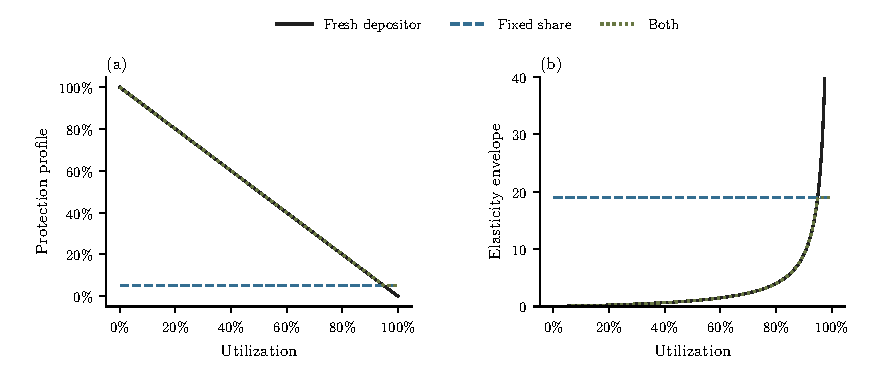
\includegraphics[width=\textwidth]{T02-envelopes.pdf}
\caption{(a) Protection profiles and (b) their elasticity envelopes. The flat target is $5\%$. Imposing both guarantees takes the larger protection profile and smaller envelope; the envelopes cross at $U=K/(1+K)=95\%$.}
\label{fig:envelope}
\end{figure}

The comparison is less obvious than it looks, because the two envelopes cross. Setting $K=U/(1-U)$ gives $U=K/(1+K)$, which is $95\%$ for $K=19$, and below that point the fresh depositor rule is the \emph{stricter} of the two while above it the flat target is. Neither guarantee implies the other, and a curve may satisfy either one alone.

Two further consequences separate this profile from a flat one. The first is that a fresh depositor guarantee cannot be offered by a curve through the origin. Applying Theorem~\ref{thm:fresh} on $[U_a,U]$ and letting $U_a\to0$ gives $R_b(U)\leq R_b(0)/(1-U)$, that is
\[
R_b(0)\geq R_b(U)\,(1-U)
\qquad\forall U<1
\]
so the base rate is bounded below by the whole curve and in particular is strictly positive. The standard below kink ramp fails for exactly this reason: being proportional to $U$ it has $\eta\equiv1$, while the envelope $U/(1-U)$ is below $1$ for every $U<\tfrac12$. A curve meant to satisfy Theorem~\ref{thm:fresh} must begin at a positive rate at zero utilization, and the example in Table~\ref{tab:cavey-example} does.

The second is that a positive anchor below full utilization places no upper bound on the rate attainable at $U=1$ when the shape between them is unrestricted. For a flat target the available rate budget $\int_O^1 K\,d\ln U$ is finite. Here the corresponding integral is $\ln((1-O)/(1-U))$, which diverges as $U\to1$. A finite maximum above the anchor can therefore be reached by following the boundary and then clamping. This does not mean arbitrary intermediate rates or a fixed set of linear segments are feasible. Section~\ref{sec:multi} discusses the additional restriction from fixed knots.

\subsection{Piecewise Linear Form}

Onchain curves are piecewise linear, and the guarantee takes an exact form on them. Take a nondecreasing segment from $(u_L,R_L)$ to $(u_H,R_H)$ with slope
\[
m=\frac{R_H-R_L}{u_H-u_L}
\]
so that $R_b(u)=R_L+m(u-u_L)$ inside it. The condition $\eta\leq u/(1-u)$ is equivalent to $m(1-u)\leq R_b(u)$, and since $R_b(u)/(1-u)$ increases along a nondecreasing segment, the binding point is the left endpoint. The segment is admissible exactly when $0\leq m\leq R_L/(1-u_L)$, and substituting the slope turns this into a rule on adjacent knots alone,
\begin{equation}
\boxed{
\frac{R_H}{R_L}
\leq
1+\frac{u_H-u_L}{1-u_L}
}
\label{eq:adjacent-rate-rule}
\end{equation}
If every segment of a continuous piecewise linear curve satisfies Equation~\ref{eq:adjacent-rate-rule}, income stays nondecreasing even for a deposit that crosses several segments, and no condition linking one segment to the next is required. A flat clamp after the final knot preserves the condition as well.

The segment rule can be checked directly on knot parameters. Appendix~\ref{app:examples} gives an admissible curve and follows a fresh deposit across its knots, separating the sign of marginal income from the level of income.

\section{A Minimal Change Construction}
\label{sec:minimal}

Return to a flat target and suppose a protocol already runs a single kink model
\[
R_{\mathrm{old}}(U)=
\begin{cases}
R_o\dfrac{U}{O}, & U\leq O\\[5pt]
R_o+m(U-O), & U>O
\end{cases}
\qquad
m=\frac{R_{\max}-R_o}{1-O}
\]
Assume $K\geq1$ and the upper branch has negative intercept, $R_o-mO<0$, as in the illustrative curve. Below the optimum $\eta=1$ and nothing needs to change. Above it $\eta_{\mathrm{old}}(U)=Um/(R_o+m(U-O))$ is largest at the kink. For $K\geq K^*$, let $U_c$ be the first utilization above $O$ at which the power law boundary catches the original branch,
\[
R_o\left(\frac{U_c}{O}\right)^K
=
R_o+m(U_c-O)
\]
For a feasible $K$ the natural construction follows the boundary only over that interval,
\[
\boxed{
R_{\mathrm{new}}(U)=
\begin{cases}
R_o\dfrac{U}{O}, & U\leq O\\[6pt]
R_o\left(\dfrac{U}{O}\right)^K, & O<U<U_c\\[7pt]
R_o+m(U-O), & U_c\leq U\leq1
\end{cases}
}
\]
preserving the curve below the kink and after the rejoin. The replacement can extend into a region where the original elasticity is already below $K$: continuity still requires the lower branch to catch up. If the original curve is admissible everywhere, no replacement interval is needed. As $\bar\alpha\to0$ the ceiling $K\to\infty$, and once $K$ exceeds the maximum original elasticity,
\[
\boxed{
\bar\alpha\to0
\quad\Longrightarrow\quad
R_{\mathrm{new}}(U)=R_{\mathrm{old}}(U)
}
\]
so the construction is better read as a constraint imposed on an existing IRM than as a proposal to replace it.

Figure~\ref{fig:borrow-curves} compares borrow and supply rates for $O=80\%$, $R_o=5\%$, $R_{\max}=100\%$ and $K=19$. The branch changes the path between the fixed endpoints while keeping both the kink rate and the maximum rate.

\begin{figure}[htbp]
\centering
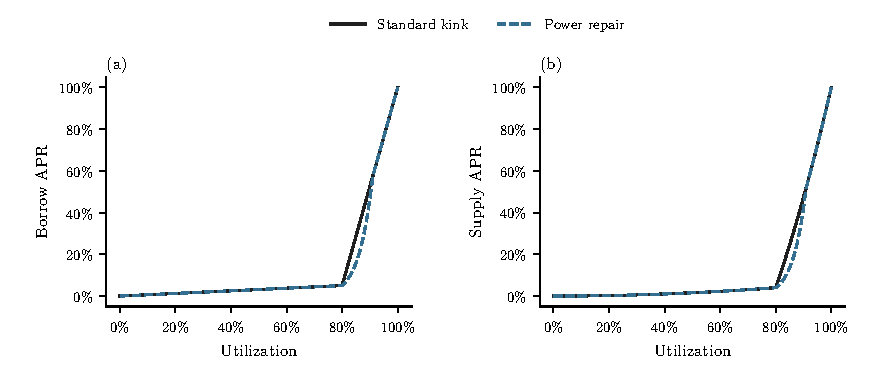
\includegraphics[width=\textwidth]{T06-single-rates.pdf}
\caption{(a) Borrow and (b) supply APR before and after the power law repair with $K=19$. The repaired branch rejoins at approximately $90.92\%$ utilization. Supply APR is $UR_b(U)$, without fees.}
\label{fig:borrow-curves}
\end{figure}

Over its replacement interval this curve pays less than the baseline at the same utilization. The benefit is that adding capital cannot reduce whole position income while the supplier remains within the protected share. Appendix~\ref{app:examples} gives a finite deposit example; preserving existing income levels requires a different pricing choice, considered below.

\section{Several Kinks and the Choice of Rates}
\label{sec:multi}

Consider a USDT market, with parameters drawn from a deployed configuration, having a $0.5\%$ minimum borrow APR, an $80\%$ main kink at $5.25\%$ APR, and a $90\%$ maximum. Further knots lie at $85\%$, $90\%$, $95\%$, $99\%$ and $99.5\%$ utilization, with rates specified in Appendix~\ref{app:multi}. The example lets us distinguish the protection a curve provides from the price levels chosen to provide it.

To protect both fresh depositors and existing suppliers up to a fixed share, impose the stronger promise at each utilization:
\[
\bar\alpha_{\mathrm{both}}(U)=\max\{\bar\alpha,1-U\}
\qquad
E_{\mathrm{both}}(U)=\min\left\{K,\frac{U}{1-U}\right\}
\]
At a $5\%$ fixed share, the fresh depositor rule binds below $95\%$ utilization and the fixed share rule above it. A power law region alone does not establish both guarantees; every retained segment must respect the tighter envelope.

With knots and maximum APR fixed, the segment constraints place a floor under preceding rates. If $r_{i+1}\leq c_i r_i$ is the applicable ratio cap, this floor is obtained by propagating the final rate backwards as $\ell_i=\ell_{i+1}/c_i$. Moving every rate to the floor can lower rates that were already acceptable. A repair that preserves them instead sets
\[
r_n^+=r_n^0
\qquad
r_i^+=\max\left\{r_i^0,\frac{r_{i+1}^+}{c_i}\right\}
\]
where $r_i^0$ denotes the baseline. This is the smallest admissible repair that never lowers a rate, so it preserves supplier income under the same principal and utilization history at a cost to borrowers. Figure~\ref{fig:repair-family} compares these choices with a mixed repair that permits increases and decreases while minimizing weighted changes to knot rates. The recursions, objective and feasibility conditions are derived in Appendix~\ref{app:multi}.

\begin{figure}[htbp]
\centering
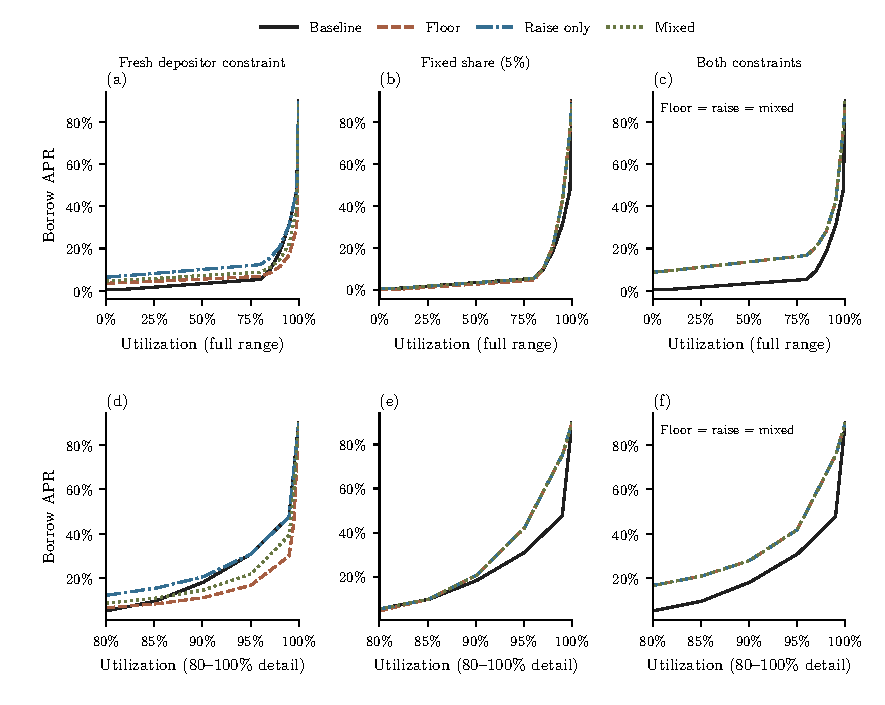
\includegraphics[width=\textwidth]{02-floor-and-repairs.pdf}
\caption{Baseline, compliant floor, raise only repair and mixed repair, at fixed knots and $90\%$ top APR. Columns impose the fresh depositor guarantee, the $5\%$ fixed share guarantee, and both. Panels (a--c) show $0$--$100\%$ utilization; panels (d--f) show the same curves enlarged over $80$--$100\%$, with no change in parameters or scenario. Under both constraints the floor is already above the baseline, so the three repairs coincide.}
\label{fig:repair-family}
\end{figure}

The implementation class matters as much as the target. On the original coarse grid, both guarantees with $5\%$ fixed share protection and a $90\%$ maximum require a base APR of at least $8.68\%$. Allowing unrestricted curved regions reduces the combined bound to $1.70\%$; requiring the analytic curve also to remain above the baseline gives approximately $1.85\%$. These are different constraints, not conflicting estimates. Appendix~\ref{app:multi} derives the bounds and shows their dependence on knot refinement.

A similar restriction appears when inserting power laws around several kinks. A branch that only lowers rates after the late $99\%$ kink reaches $57.65\%$ at full utilization and cannot retain the original $90\%$ maximum. Preserving that maximum requires changing rates earlier. The analytic constructions in Appendix~\ref{sec:analytic} locate these replacement regions directly and distinguish repairs that never raise rates from those that never lower them.

\section{Income Levels and Accumulated Interest}
\label{sec:earnings}

Whether a depositor earns more over a holding period depends on the rates they encounter and the capital they hold at each point, rather than on the sign of the deposit derivative alone. For prescribed principal $b(t)$ and utilization $U(t)$, with a constant withheld fraction $f$, accumulated interest is
\[
A(H)=\int_0^H(1-f)b(t)U(t)R_b(U(t))\,dt
\]
where time is measured in years. Comparing two curves on identical histories gives
\[
\Delta A(H)=\int_0^H(1-f)b(t)U(t)
\left[R_1(U(t))-R_0(U(t))\right]dt
\]
A raise only repair therefore cannot reduce accumulated supplier interest under the same history; a lower only repair cannot increase it. A mixed change depends on where the depositor spends time and how much capital is present there. None of these statements predicts the history after borrowers and suppliers respond to new prices.

Each comparison below holds borrowings fixed and replays an identical utilization path under every curve, which isolates the effect of pricing. That isolation is itself an assumption: a curve charging borrowers more would in practice face different borrowing, and so a different utilization path from the one priced here. The figures report what each curve would have paid on a given history, not what a market would do once prices move.

The examples use a constant $5\%$ carveout from borrower interest, with interest paid out rather than compounded into the position. They evaluate the continuous curves and omit additional fees, incentives, losses and token rounding, so differences come entirely from the prescribed rate functions and market histories.

\begin{figure}[htbp]
\centering
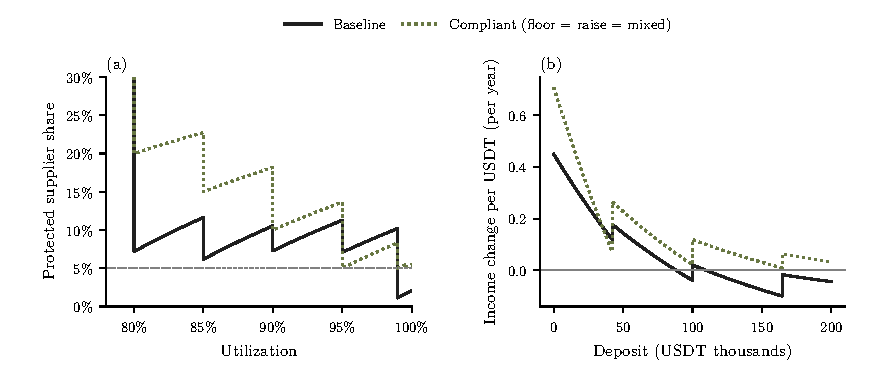
\includegraphics[width=\textwidth]{04-protection-and-marginal-income.pdf}
\caption{Both guarantees on the fixed knots. (a) Actual protected share, with the $5\%$ target marked. (b) Marginal whole position income for a fresh depositor entering a pool with $1$ million USDT supply and $990{,}000$ USDT of fixed borrowing. The floor, raise only and mixed curves coincide here. Their marginal income stays nonnegative across the crossed knots; the baseline's does not.}
\label{fig:multi-marginal}
\end{figure}

First take a $10{,}000$ USDT depositor in a pool with $1$ million USDT supply. They hold for one year while utilization moves linearly through $80\%$, $95\%$, $99.5\%$, $85\%$ and $80\%$ on days $0$, $90$, $180$, $270$ and $365$. Under the fresh depositor guarantee alone, the floor pays about $1{,}287$ USDT, the raise only repair $2{,}231$, and the mixed repair $1{,}680$, against $1{,}983$ under the baseline. All three repairs obey the same guarantee and keep the same maximum. Their different earnings come from the choice of rate levels.

\begin{figure}[htbp]
\centering
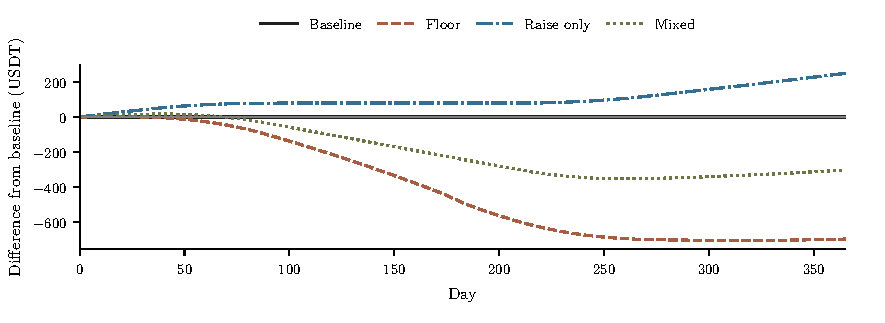
\includegraphics[width=\textwidth]{07-fresh-pricing-choice.pdf}
\caption{Fresh depositor guarantee only, on the stated single deposit history. (a) Accumulated interest and (b) difference from baseline. A compliant floor is not the same choice as a repair that preserves existing rates. Principal is excluded from interest.}
\label{fig:fresh-lifecycle}
\end{figure}

Higher supplier earnings on an unchanged history are funded by borrower payments. Since this depositor owns $1\%$ of the pool, each additional unit of aggregate borrower interest contributes $0.0095$ units to the depositor after the carveout. The guarantee controls the response to adding capital; it does not determine whether the price level is desirable for either side of the market.

Appendix~\ref{app:histories} considers repeated deposits, stronger protection targets and different utilization exposures. Those comparisons retain identical histories across curves to isolate pricing. Predicting how demand, liquidity or risk responds to repricing requires a separate model and is outside the claim here.

\section{Checking the Constraint Onchain}
\label{sec:onchain}

Onchain implementations represent rate curves with linear segments rather than evaluating fractional powers or exponentials, and the flat share constraint can be checked directly in that form. For a segment from $(u_i,r_i)$ to $(u_{i+1},r_{i+1})$ with slope $m_i$,
\[
R_b(U)=r_i+m_i(U-u_i)
\qquad
\eta(U)=\frac{Um_i}{R_b(U)}
\]
and elasticity is monotone across a positive linear segment, so checking both endpoints bounds it over the whole segment. Writing $\Delta r=r_{i+1}-r_i$ and $\Delta U=u_{i+1}-u_i$, the endpoint condition can be put in a form with no division at all,
\[
\boxed{
U\Delta r\leq Kr\Delta U
}
\]
which suits fixed point integer arithmetic and imposes the elasticity requirement on an otherwise standard piecewise linear IRM. It belongs in parameter validation rather than in the rate computation, so the hot path is untouched.

The check applies to the curve actually implemented. Replacing an analytic boundary with straight chords can violate its elasticity ceiling, and integer evaluation needs its own rounding headroom. Appendix~\ref{app:implementation} gives the chord example and the scope of the numerical checks; a derivative condition for the continuous curve is not by itself a guarantee after token rounding.

\section{Conclusion}

The condition $\alpha(1+\eta)\leq1$ separates the supplier's pool share from the rate curve's response to utilization, and turning it into a curve constraint needs exactly one economic input: the protection profile $\bar\alpha(U)$. When the condition fails, a supplier's best response is to withdraw until it holds, which raises utilization in the state where the pool can least afford it. Everything else follows from the choice of profile, through the envelope $E=(1-\bar\alpha)/\bar\alpha$, the constraint $\eta\leq E$, and the integral bound of Theorem~\ref{thm:family} describing the whole admissible family.

The two rules are particular profiles. A flat target gives the constant ceiling $K$, the power law boundary and the endpoint obstruction $K^*$. Protecting every fresh depositor gives the profile $1-U$, the hyperbolic boundary and the adjacent rate rule of Equation~\ref{eq:adjacent-rate-rule}. Its rate budget up to full utilization is unbounded when the shape is unrestricted, but fixed knots impose additional bounds. Neither guarantee contains the other; their intersection takes the smaller envelope and has a finite combined endpoint budget.

The multiple kink comparison separates the guarantee from the pricing decision. A minimum rate curve need not preserve supplier income. A repair that never lowers rates does preserve it under identical balances and market histories, with the increase paid by borrowers. Analytic replacement regions can require much less repricing than a coarse fixed knot implementation, and a late power branch need not rejoin before the original maximum. These are reasons to state the fixed endpoints, allowed knot changes and protection target together.

On a piecewise linear curve the constraint is checked at segment endpoints. Smoothness is a further choice: continuous elasticity removes jumps in the advertised protection at the cost of headroom above $K^*$. The mathematical result is deposit income monotonicity within the chosen profile. Whether the resulting prices improve participation or market outcomes is a separate question.

\clearpage
\appendix
\setcounter{figure}{0}
\renewcommand{\thefigure}{A\arabic{figure}}
\renewcommand{\theHfigure}{appendix.\arabic{figure}}
\section{Boundary Curves and Deposit Examples}
\label{app:examples}

The examples in this appendix illustrate the two guarantees without introducing additional assumptions into the main result. Boundary curves describe rate ceilings from a specified anchor; income comparisons also depend on the rates chosen within those ceilings.

\begin{figure}[htbp]
\centering
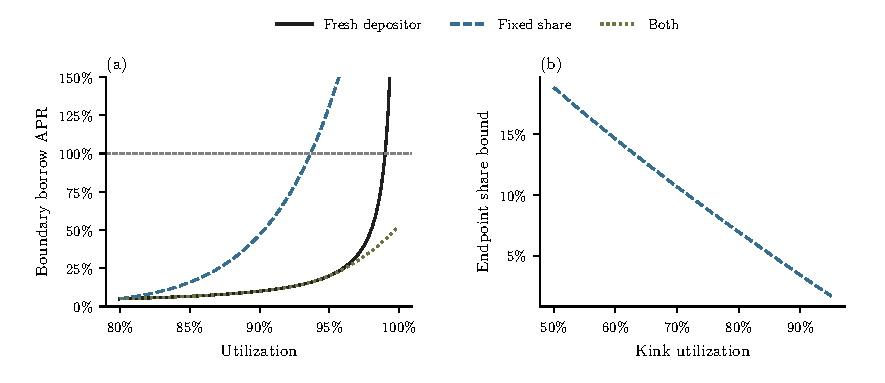
\includegraphics[width=\textwidth]{T03-boundaries-endpoints.pdf}
\caption{(a) Boundary curves anchored at $(80\%,5\%)$, with a $100\%$ rate reference. The combined boundary uses the smaller envelope and cannot reach that reference from this anchor. (b) The fixed share endpoint bound as kink utilization varies, with kink APR $5\%$ and maximum APR $100\%$. These are bounds rather than proposed rate curves.}
\label{fig:boundary-curves}
\end{figure}

\subsection{A Fresh Depositor Crossing Several Knots}

The following curve satisfies the adjacent rate rule from Section~\ref{sec:fresh} and retains an increasing emergency branch near full utilization.

\begin{table}[htbp]
\centering
\caption{A piecewise linear borrow rate curve satisfying deposit monotonicity.}
\label{tab:cavey-example}
\begin{tabular}{@{}rrrr@{}}
\toprule
Segment & Rate ratio & Maximum ratio & Result \\
\midrule
$0\%\!\to\!80\%$       & 1.800 & 1.800 & tight \\
$80\%\!\to\!90\%$     & 1.500 & 1.500 & tight \\
$90\%\!\to\!95\%$     & 1.481 & 1.500 & valid \\
$95\%\!\to\!98\%$     & 1.600 & 1.600 & tight \\
$98\%\!\to\!99.5\%$   & 1.750 & 1.750 & tight \\
$99.5\%\!\to\!99.99\%$ & 1.964 & 1.980 & valid \\
\bottomrule
\end{tabular}
\end{table}

\begin{figure}[htbp]
\centering
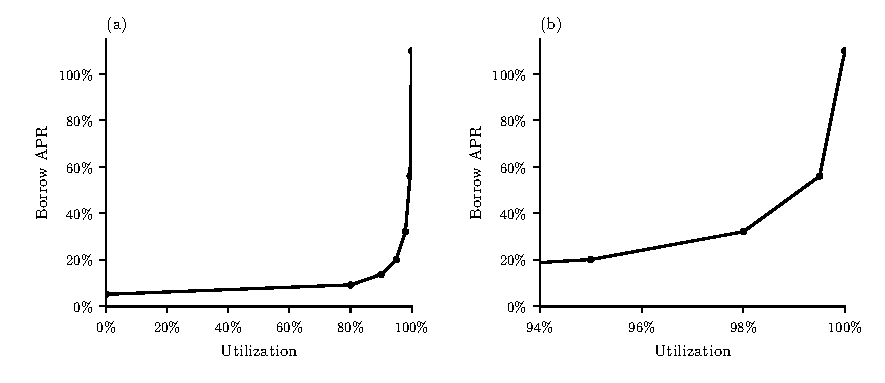
\includegraphics[width=\textwidth]{T04-piecewise-example.pdf}
\caption{A piecewise linear curve with knots at $0\%$, $80\%$, $90\%$, $95\%$, $98\%$, $99.5\%$ and $99.99\%$ utilization and borrow APRs of $5\%$, $9\%$, $13.5\%$, $20\%$, $32\%$, $56\%$ and $110\%$, followed by a flat extension to the endpoint at $100\%$ utilization (also marked). Every segment satisfies Equation~\ref{eq:adjacent-rate-rule}, and the nonzero rate at the origin is forced by the base rate bound.}
\label{fig:deposit-monotonic-curve}
\end{figure}

Figure~\ref{fig:fresh-income} shows the guarantee doing its work. A fresh depositor arrives at a pool with \$10 million of supply and \$9.99 million of fixed borrowing, and deposits until utilization reaches $85\%$. The path crosses the knots at $99.5\%$, $98\%$, $95\%$ and $90\%$. Under Table~\ref{tab:cavey-example}, income rises over the whole path. Under the standard kinked curve of Section~\ref{sec:failure}, income peaks and then falls; its marginal dollar turns negative at a deposit of about \$1.17 million.

Within each tight linear segment the marginal income approaches zero as the depositor moves towards its left endpoint. It reaches zero there for the most demanding start $u_0=1$. For the illustrated start $u_0=0.999$, the margin is small but positive. The segment rule is tight for the global guarantee, not necessarily for every individual deposit path.

\begin{figure}[htbp]
\centering
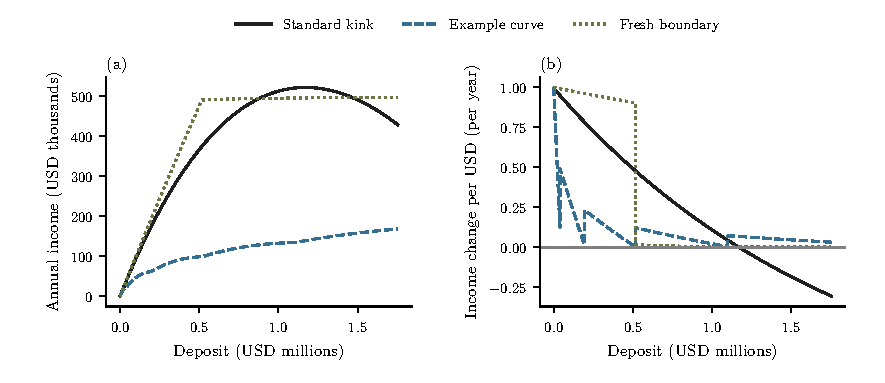
\includegraphics[width=\textwidth]{T05-fresh-income.pdf}
\caption{(a) Annualized income and (b) marginal income along the fresh depositor path. The standard kink has zero base rate. Table~\ref{tab:cavey-example} and the clamped fresh boundary have $5\%$ base rates; the table reaches $110\%$ maximum APR, while the other two reach $100\%$. These different rate levels are stated explicitly: the comparison illustrates the guarantee, not a common endpoint repair.}
\label{fig:fresh-income}
\end{figure}

The curve in Table~\ref{tab:cavey-example} pays less than the kinked one over this path, ending at about \$168{,}000 against \$428{,}000. This difference reflects the chosen rates rather than an unavoidable cost of the guarantee: at $95\%$ utilization it charges $20\%$ where the rule would allow $100\%$.

The third curve takes equality in Theorem~\ref{thm:fresh} from a base rate $r_0=5\%$, giving $R_b(U)=\min\{r_0/(1-U),100\%\}$. It charges about $33\%$ at $85\%$ utilization against the standard curve's $29\%$, reaches its maximum at $95\%$, and ends the path at about \$497{,}000 a year. It has the same maximum as the standard curve but a higher base. The guarantee constrains percentage sensitivity; it does not fix the price level or establish that every compliant curve earns more.

Below the clamp, the boundary gives
\[
\frac{dI}{dx}=\frac{r_0u^2(1-u_0)}{u_0(1-u)^2}
\]
This vanishes when $u_0=1$ and is positive for the illustrated start. A boundary means equality in the worst case constraint, not indifference for every depositor.


\subsection{An Existing Supplier Under a Power Law Repair}

For a supplier who begins above the kink and grows to $5\%$ of final supply, the constrained curve holds both total income and its marginal change nonnegative over the whole deposit path, while the original curve reduces total income over part of it.

What this buys needs stating precisely. This particular repair lies below the original over the replaced interval, so it charges borrowers less and pays suppliers less at the same state. Figure~\ref{fig:partial-supplier-income} starts with a \$100{,}000 supplier in a \$10 million pool at $85\%$ utilization and ends when the supplier owns $5\%$. The original income eventually falls while the repaired income remains nondecreasing. This is an income direction guarantee, not a claim of higher earnings. Other repairs can raise rates instead, as discussed in Section~\ref{sec:multi}.

\begin{figure}[htbp]
\centering
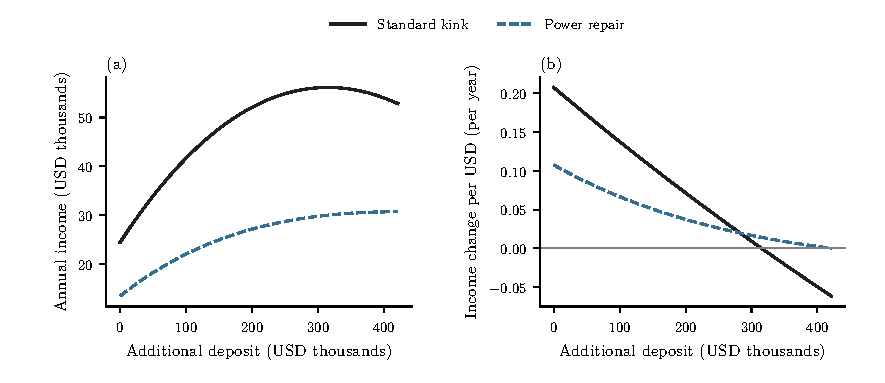
\includegraphics[width=\textwidth]{T07-single-income.pdf}
\caption{(a) Annualized income and (b) marginal income for the existing supplier, with \$8.5 million of fixed borrowing. The path ends at $5\%$ ownership. The repaired marginal income reaches zero at that boundary; the original becomes negative sooner.}
\label{fig:partial-supplier-income}
\end{figure}


\clearpage
\section{Constructions for Several Kinks}
\label{app:multi}

Assume a multiple kink USDT market with a $0.5\%$ minimum borrow APR, an $80\%$ main kink at $5.25\%$ APR, and a $90\%$ maximum. Below the main kink the rate is $\max\{0.5\%,5.25\%\,U/0.8\}$. Above it, straight segments connect the knots in Table~\ref{tab:multi}. These are illustrative inputs, not measurements of a live market or a proposed parameter update. All fixed-knot recursions below use the complete grid: $0\%$, the exact floor crossing $U=0.005(0.8)/0.0525\approx7.619\%$, and the seven utilizations in Table~\ref{tab:multi}.

\begin{table}[htbp]
\centering
\caption{The illustrative multiple kink rate curve. The floor meets the initial ramp at approximately $7.619\%$ utilization.}
\label{tab:multi}
\begin{tabular}{@{}rrrrrrrr@{}}
\toprule
Utilization & $80\%$ & $85\%$ & $90\%$ & $95\%$ & $99\%$ & $99.5\%$ & $100\%$ \\
\midrule
Borrow APR & $5.25\%$ & $9.4875\%$ & $17.9625\%$ & $30.675\%$ & $47.625\%$ & $68.8125\%$ & $90\%$ \\
\bottomrule
\end{tabular}
\end{table}

\begin{figure}[htbp]
\centering
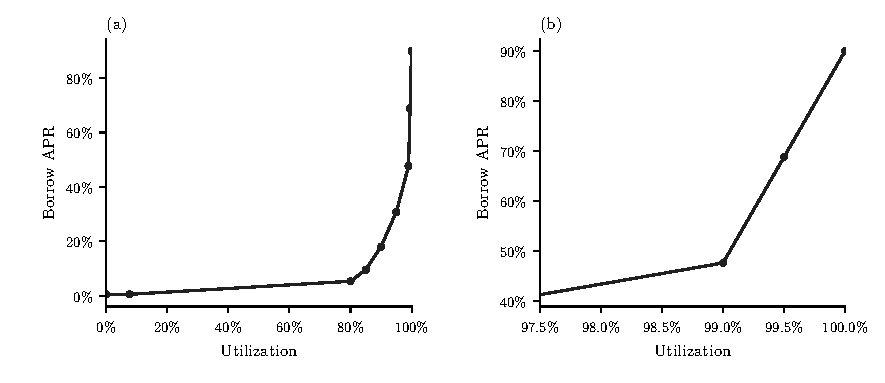
\includegraphics[width=\textwidth]{01-usdt-baseline.pdf}
\caption{The illustrative multiple kink curve: (a) full utilization range and (b) the final segments. The interval from $99\%$ to $99.5\%$ carries $21.1875$ percentage points of borrow APR.}
\label{fig:multi-baseline}
\end{figure}

\subsection{One Guarantee or Both}

Protecting both an incoming depositor and an existing holder up to a fixed share requires the stronger promise at each utilization. The required protected share is therefore the larger profile, and the allowed elasticity the smaller envelope:
\[
\bar\alpha_{\mathrm{both}}(U)=\max\{\bar\alpha,1-U\}
\qquad
E_{\mathrm{both}}(U)=\min\left\{K,\frac{U}{1-U}\right\}
\]
For $\bar\alpha=5\%$, the fresh depositor rule binds below $95\%$ utilization and the fixed share rule above it. Adding a power law region does not by itself establish both guarantees. Every retained segment must satisfy whichever envelope is tighter there.

On a linear segment $[u_i,u_{i+1}]$, write $\Delta u_i=u_{i+1}-u_i$. The fresh depositor cap on $r_{i+1}/r_i$ is
\[
c_i^{\mathrm{fresh}}=1+\frac{\Delta u_i}{1-u_i}
\]
Checking the fixed share condition at both endpoints gives
\[
c_i^{\mathrm{fixed}}=\min\left\{
1+\frac{K\Delta u_i}{u_i},\
\frac{u_{i+1}}{u_{i+1}-K\Delta u_i}
\right\}
\]
where a term imposes no restriction if $u_i=0$ in the first denominator or the second denominator is nonpositive. Taking $c_i=\min\{c_i^{\mathrm{fresh}},c_i^{\mathrm{fixed}}\}$ imposes both guarantees, with the complete segment constraint $r_i\leq r_{i+1}\leq c_i r_i$.

\subsection{Rate Floors and Repair Choices}

If a market must still reach its existing maximum, limiting the increase on each segment places a lower bound on the rates leading up to it. For fixed knots and final rate $r_n$, this bound follows by setting $\ell_n=r_n$ and working backwards:
\[
\ell_i=\frac{\ell_{i+1}}{c_i}
\]
An unbounded cap gives a zero lower bound. Every feasible curve with these knots and top rate must lie above the resulting floor, but moving all rates down to it can reduce supplier income even where the baseline was already compliant. A protocol that wants to preserve that income can instead require each repaired rate to remain at least as high as its baseline value.

Writing those baseline rates as $r_i^0$, the least such repair is
\[
r_n^+=r_n^0,\qquad
r_i^+=\max\left\{r_i^0,\frac{r_{i+1}^+}{c_i}\right\}
\]
Because the baseline is nondecreasing, the backwards recursion satisfies both segment inequalities. Any admissible curve above the baseline must meet the same backwards bounds, making this the pointwise smallest repair that preserves existing rates. Supplier income cannot fall under an unchanged market history, although the higher rates increase borrower costs.

The opposite choice fixes the base and never raises a baseline rate:
\[
r_0^-=r_0^0,\qquad
r_{i+1}^-=\min\{r_{i+1}^0,c_i r_i^-\}
\]
This is the greatest admissible curve below the baseline, but its top rate is not fixed. Keeping the original top while never raising a rate is infeasible whenever the baseline falls below the corresponding fixed top floor.

Allowing both increases and decreases gives a third pricing choice. The mixed repair in the figures minimizes $\sum_i w_i(r_i-r_i^0)^2$ over feasible knot rates with the top held fixed, using trapezoidal utilization weights $w_i$. This objective measures changes to the knot parameters; it does not optimize borrower or supplier welfare, nor is it the exact integral of squared curve error.



For the fresh depositor rule, the fixed top floor has base APR $3.47\%$, while preserving every baseline rate requires $6.39\%$. Under both guarantees the minimum base is $8.68\%$ on these knots, and the floor, raise only and mixed repairs coincide. The numbers describe this knot grid; they are not universal minimum prices for monotonicity. A repair that never raises the baseline instead reaches only $12.04\%$ maximum APR under the fresh rule and $4.82\%$ under both, rather than $90\%$.

\begin{figure}[htbp]
\centering
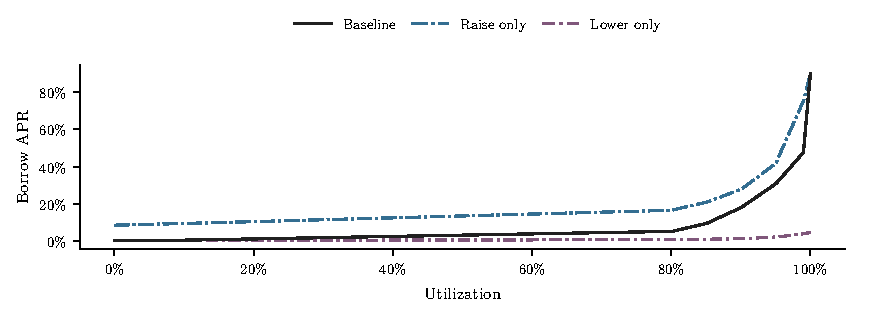
\includegraphics[width=\textwidth]{03-direction-of-repair.pdf}
\caption{Both guarantees: (a) APR changes from baseline and (b) resulting rates. Raise only retains the $90\%$ top and coincides with the floor and mixed repair. Lower only retains the original base and never raises a rate, but must lower the maximum. The different endpoint choices are part of the comparison.}
\label{fig:repair-direction}
\end{figure}

\subsection{Power Law Regions on a Multiple Kink Curve}
\label{sec:analytic}

With several kinks, a rate lowering power branch may fail to catch the original curve before full utilization even when the main kink and maximum satisfy the global endpoint bound. Retaining low rates at intermediate knots can leave too little utilization range for the final increase, so preserving the maximum may require raising rates before the offending segment.

For the constructions in this subsection, assume a continuous, nondecreasing piecewise linear baseline with strictly positive base rate, as in the illustrative curve. This ensures the running-infimum minorant remains positive. For the fixed-share envelope, a baseline with a positive-slope first segment through the origin is also permitted when $K\geq1$; when $K<1$ its running-infimum minorant is identically zero and is outside the positive-rate class.

These replacement regions can be constructed by measuring the baseline relative to the fastest rate increase allowed by the guarantee. Let $F$ be a positive boundary function on $U>0$, with $F'/F=E(U)/U$, and write $q_0(U)=R_0(U)/F(U)$. Admissibility requires $R/F$ to be nonincreasing: once the rate has fallen behind its boundary, it cannot catch up by exceeding the envelope later. The largest admissible curve below the baseline and the smallest one above it are therefore
\[
\boxed{
\begin{aligned}
R_-(U)&=F(U)\inf_{0<v\leq U}q_0(v)\\
R_+(U)&=F(U)\sup_{U\leq v\leq1}q_0(v)
\end{aligned}
}
\]
Values at zero are taken by continuity. The first construction preserves as much borrower pricing as possible without raising any rate; the second preserves supplier pricing by raising only what the constraint requires.

\begin{proof}
The envelope condition is equivalent to $R/F$ being nonincreasing. Any admissible minorant therefore satisfies $R(U)/F(U)\leq q_0(v)$ for every $v\leq U$, giving the first bound. The running infimum is itself nonincreasing and meets that bound. The majorant follows by the same argument with future points and a running supremum. On a piecewise linear nondecreasing baseline, the resulting curve follows either the baseline or a constant multiple of $F$. Both are nondecreasing; the construction is continuous at contacts. Thus the bounds also belong to the rate class assumed here.
\end{proof}

For fixed share protection, $F(U)=U^K$, so the replacement intervals are power laws. On the illustrative multiple kink curve with $K=19$, the minorant first departs at $99\%$ utilization and reaches only $57.65\%$ APR at full utilization. It cannot retain the $90\%$ maximum. The majorant retains that maximum by raising rates earlier, while still preserving the original base and $80\%$ kink rate. The formulas include interior extrema of $q_0$ on each original segment; checking the knot values alone is not sufficient for the running supremum.

\begin{figure}[htbp]
\centering
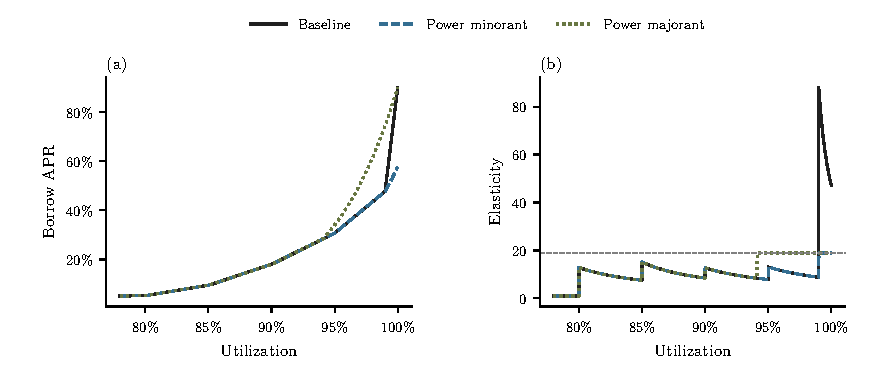
\includegraphics[width=\textwidth]{M08-analytic-power.pdf}
\caption{Analytic fixed share repairs with $K=19$: (a) borrow APR and (b) elasticity. The power minorant never raises rates but misses the original maximum. The power majorant preserves the maximum and raises the rates needed to reach it. The horizontal line marks the elasticity ceiling.}
\label{fig:analytic-power}
\end{figure}

To impose both guarantees, let $t=K/(K+1)$ and normalize the combined boundary at the origin:
\[
F(U)=
\begin{cases}
(1-U)^{-1},&0\leq U\leq t\\[3pt]
(K+1)(U/t)^K,&t<U\leq1
\end{cases}
\]
The same construction then uses hyperbolic regions below $t$ and power law regions above it, retaining the baseline wherever contact permits. This is distinct from the fixed knot linear implementation. The combined analytic majorant has base APR approximately $1.85\%$ and keeps the $90\%$ maximum, compared with $8.68\%$ for the coarse fixed knot repair.

\begin{figure}[htbp]
\centering
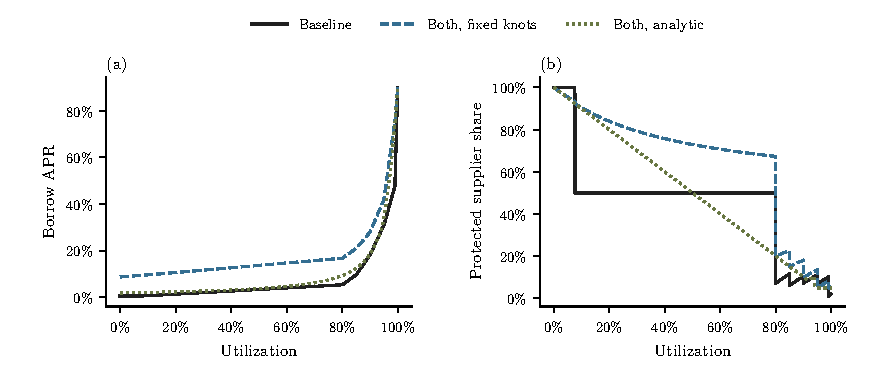
\includegraphics[width=\textwidth]{M09-analytic-combined.pdf}
\caption{Both guarantees, with $5\%$ fixed share protection. The fixed knot and analytic curves are the least repairs nowhere below the same baseline in their respective classes. (a) Borrow APR. (b) Actual protected share. The analytic curve can place new contacts and use curved regions; it is not restricted to the original knot grid.}
\label{fig:analytic-combined}
\end{figure}

\subsection{The Cost of Keeping the Knots}

The combined envelope has a finite budget even though the fresh depositor envelope alone does not. With no restriction on knot placement, its fixed top base bound is
\[
\boxed{
R_b(0)\geq\frac{R_{\max}}{F(1)}
=\frac{R_{\max}t^K}{K+1}
}
\]
For $K=19$ and $R_{\max}=90\%$, this is $1.70\%$. It is attained by a scaled combined boundary. That curve need not lie above the baseline; preserving the baseline raises the bound to the $1.85\%$ found above.

Figure~\ref{fig:knot-sensitivity} subdivides each original segment and recalculates the linear floor. At $64$ subsegments per original segment, its combined base falls from $8.68\%$ to $1.80\%$, approaching the continuous bound. Under the fresh rule alone it falls towards zero as more of the rate increase can be concentrated near full utilization. A finite set of linear knots and the continuous admissible family are different design spaces, and their bounds should not be interchanged.

\begin{figure}[htbp]
\centering
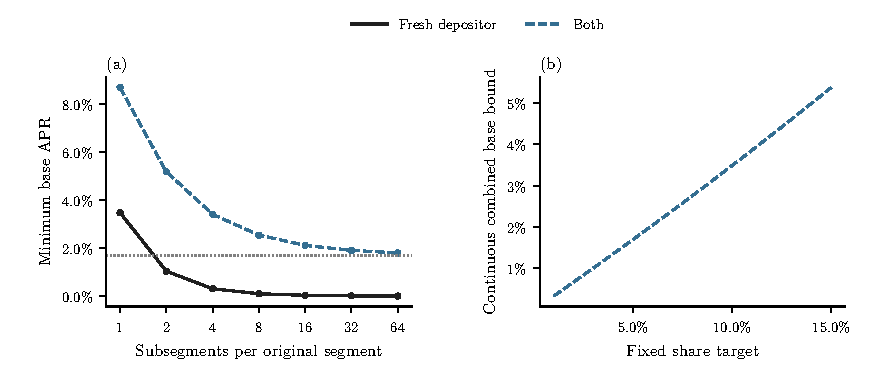
\includegraphics[width=\textwidth]{M10-knot-sensitivity.pdf}
\caption{(a) Minimum base APR at a fixed $90\%$ maximum as every original interval is subdivided equally. The dotted reference is the continuous combined bound, not a floor for the fresh only rule. (b) The continuous combined base bound as the fixed share target varies. These floors do not additionally require staying above the baseline.}
\label{fig:knot-sensitivity}
\end{figure}


\clearpage
\section{Additional Interest Scenarios}
\label{app:histories}

The histories below extend Section~\ref{sec:earnings}. They use the same $5\%$ constant carveout, pay interest out rather than compounding it, and prescribe identical principal and utilization paths for each rate curve.

Under both guarantees on the fixed knots, the three repairs coincide and pay approximately $3{,}165$ USDT on the deposit history specified in Section~\ref{sec:earnings}. A second example begins with a $10{,}000$ USDT depositor in a pool holding $1$ million USDT against $990{,}000$ borrowed. The depositor adds $20{,}000$ on each of days $60$, $120$, $180$, $240$ and $300$, while borrowing remains fixed. Annual interest is about $19{,}667$ USDT under the combined repair and $13{,}453$ under the baseline. Ownership eventually exceeds $5\%$; the local guarantee still has to be read from the protection profile rather than inferred from the label of the curve.

\begin{figure}[htbp]
\centering
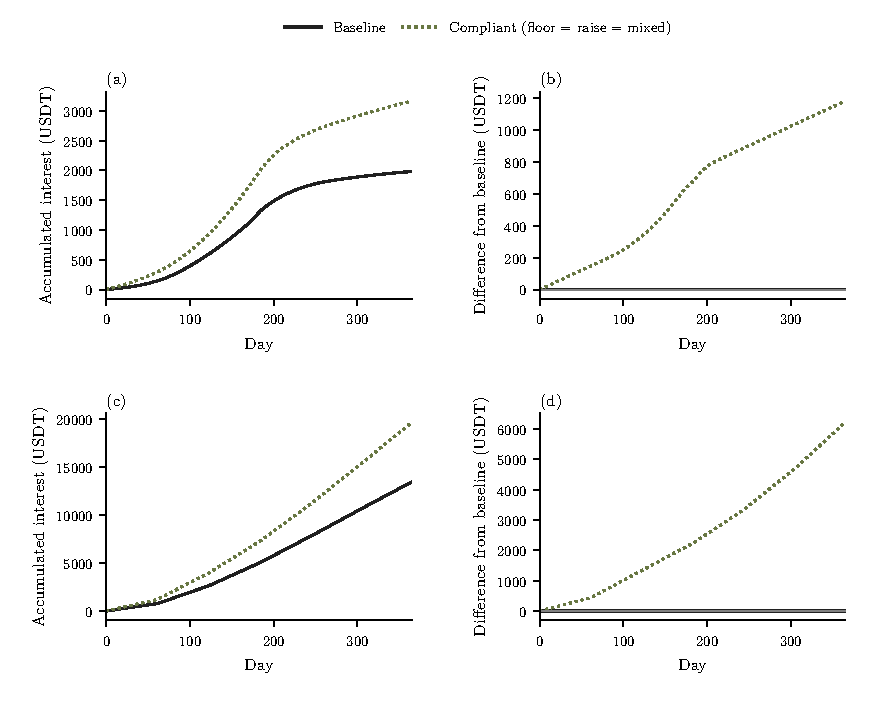
\includegraphics[width=\textwidth]{05-lifecycle-comparison.pdf}
\caption{Both guarantees on fixed knots. Top row: the single deposit history. Bottom row: repeated additions into fixed borrowing. Left: accumulated interest. Right: difference from baseline. All curves use identical principal and utilization histories, a $5\%$ carveout and no compounding. Exit at the end returns principal separately.}
\label{fig:both-lifecycle}
\end{figure}

Higher supplier income on an unchanged history is funded by higher borrower payments. The single deposit supplier owns $1\%$ of the pool, so each additional unit of aggregate borrower interest contributes $0.0095$ units to that supplier after the carveout. Figure~\ref{fig:protection-cost} follows this transfer as the fixed share target varies, retaining the fresh guarantee, original knots and maximum; it measures the resulting prices rather than their effect on welfare.

\begin{figure}[htbp]
\centering
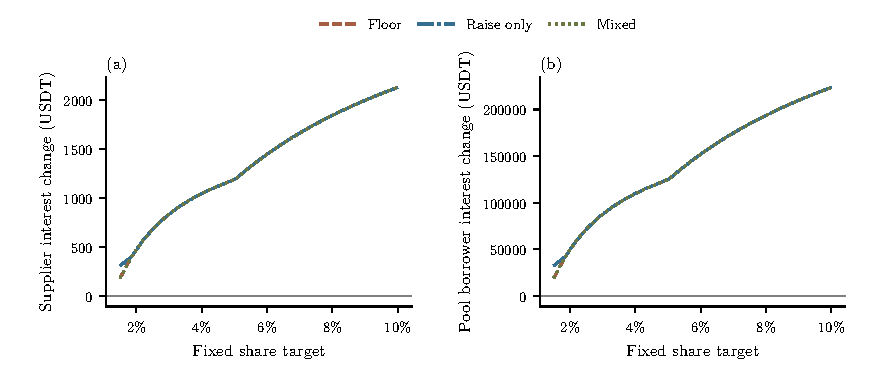
\includegraphics[width=\textwidth]{06-protection-cost.pdf}
\caption{Both guarantees as the fixed share target varies. (a) Annual supplier interest change and (b) aggregate borrower interest change, on the single deposit history. The repairs coincide over much of this range. With fixed $1\%$ ownership and a $5\%$ carveout, panel (a) is $0.0095$ times panel (b).}
\label{fig:protection-cost}
\end{figure}

To test dependence on utilization exposure, Figure~\ref{fig:exposure} allocates a year between $80\%$ and $99\%$ utilization for the same $10{,}000$ USDT principal. The fresh only floor can gain at low utilization and lose at high utilization, whereas the raise only repair cannot lose under any such mix. The analytic power minorant and majorant have the corresponding sign restrictions. These comparisons distinguish conclusions that follow from the direction of rate changes from outcomes that depend on a chosen history.

\begin{figure}[htbp]
\centering
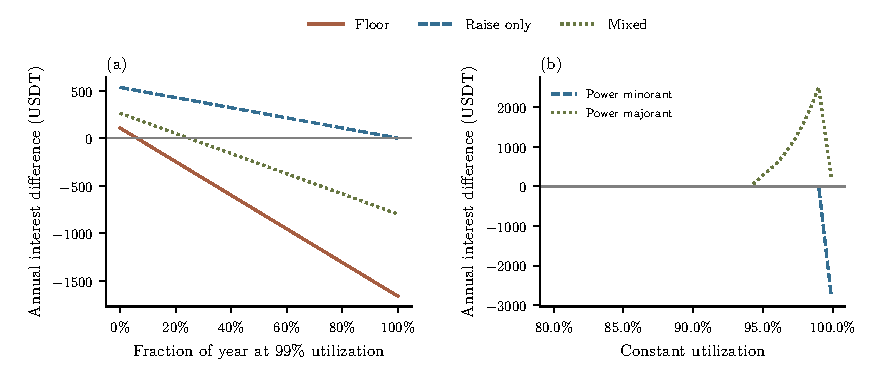
\includegraphics[width=\textwidth]{M11-exposure-sensitivity.pdf}
\caption{Sensitivity to utilization exposure. (a) Fresh only fixed knot repairs: a year is split between $80\%$ and $99\%$ utilization, with the high utilization fraction on the horizontal axis. The top legend applies to this panel. (b) Fixed share analytic power repairs: annual interest differences at a constant utilization, with a separate legend. Both panels hold principal at $10{,}000$ USDT and use a $5\%$ carveout.}
\label{fig:exposure}
\end{figure}

The sign condition holds independently of these examples, while the accumulated earnings depend on their specified histories. Predicting borrowing demand, liquidity, utilization or default risk after repricing requires a separate model. At the limiting case of $100\%$ ownership, supplier income equals total borrower interest, so any strictly increasing rate curve makes added supply reduce income at fixed borrowing, as shown in Appendix~\ref{app:full}.


\clearpage
\section{Discretisation and Numerical Checks}
\label{app:implementation}

One caveat applies to any discretisation of a smooth boundary. Sampling the constant elasticity boundary at two knots replaces it by a chord whose slope is the average of the slopes it spans, so the chord is steeper than the boundary at the segment's left endpoint. That endpoint is where elasticity binds, since the chord of a convex curve has negative intercept and $\eta$ therefore decreases across the segment, and the sampled curve is more elastic there than the boundary it was drawn from. Sampling $R_o(U/O)^{19}$ at $80\%$ and $90\%$, for instance, gives a segment whose elasticity at $80\%$ is about $67$. A ceiling imposed on a sampled curve has to be chosen with considerable headroom, or the knots placed close enough together that the chords track the boundary.

\begin{figure}[htbp]
\centering
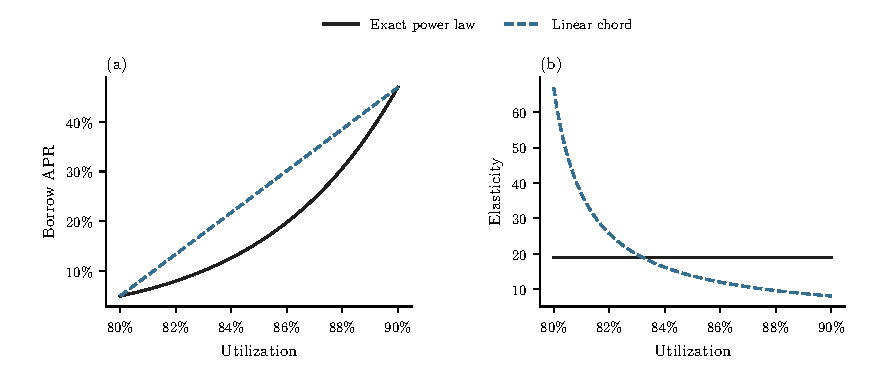
\includegraphics[width=\textwidth]{A02-discretization.pdf}
\caption{(a) A constant elasticity power law and its chord between $80\%$ and $90\%$ utilization. (b) Their elasticities. Matching endpoint rates does not preserve the ceiling between the endpoints.}
\label{fig:discretization}
\end{figure}

The checks above concern the continuous rate represented by the parameters. Integer evaluation introduces small steps, for which a derivative is not defined. In the illustrative multiple kink calculation, evaluating the integer formula at all $1{,}000{,}001$ utilization ticks differs from the rational curve by less than $10^{-6}$ in decimal APR. That agreement is not a proof of exact transaction level monotonicity after all token and interest rounding. An implementation needs rounding headroom and finite increment checks at its own precision, and a shared global weight table may not express an arbitrary per market repair.


\clearpage
\section{Smooth Constructions}
\label{sec:smooth}

A protocol may also want the advertised protected share to vary continuously with utilization. This requires a continuous elasticity profile and imposes an additional cost beyond the deposit monotonicity constraint.

The minimal change construction is continuous in the rate but not in its derivative: below the kink the slope is $R_o/O$ while the power branch leaves at $KR_o/O$, so unless $K=1$ the two disagree, and the same mismatch occurs in reverse at $U_c$. That is worth something more than tidiness, because the protected share is computed from elasticity,
\[
\alpha_{\mathrm{safe}}(U)=\frac{1}{1+\eta(U)}
\]
and therefore inherits every discontinuity of it. Under the minimal change curve $\alpha_{\mathrm{safe}}$ falls from $\tfrac12$ to $1/(1+K)$ at a single point, so a supplier holding $30\%$ of the pool is protected at $U=O-\varepsilon$ and unprotected at $U=O+\varepsilon$, and the guarantee the protocol advertises jumps while the state variable it depends on moves continuously.

\begin{figure}[htbp]
\centering
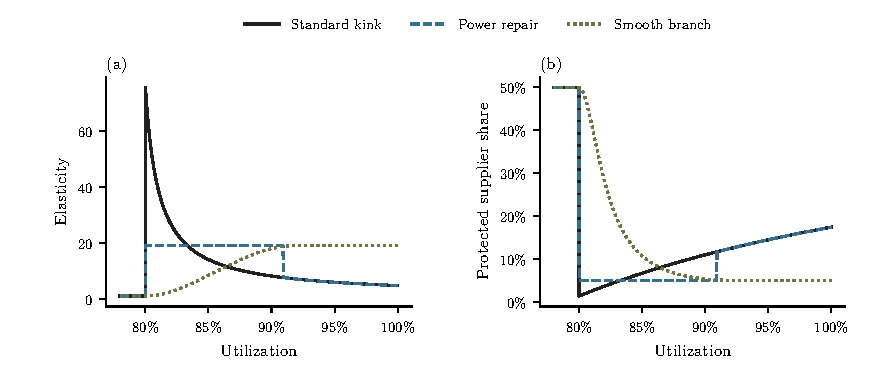
\includegraphics[width=\textwidth]{A03-smooth-protection.pdf}
\caption{(a) Elasticity and (b) protected share for the standard kink, the minimal power repair and a smooth branch. The repaired curves satisfy $K=19$; the standard kink does not. The power repair jumps in protected share, while the smooth branch changes continuously.}
\label{fig:protected-share}
\end{figure}

Removing the jump means asking elasticity itself to vary continuously, and Section~\ref{sec:family} already supplies the means. Choose a continuous profile $\eta$ on $[O,1]$ that starts at the initial value $\eta(O)=\eta_0$, stays below a ceiling $K$, and recover the rate from it,
\[
R_b(U)=R_o\exp\left(\int_O^U\frac{\eta(v)}{v}\,dv\right)
\]
Then $R_b'=\eta R_b/U$ is continuous, the branch is $C^1$, and matching $\eta_0$ at the kink makes the assembled curve $C^1$ across the join. Appendix~\ref{app:smoothstep} carries out the construction explicitly for one such family.

The ceiling cannot be taken all the way down to the endpoint bound, however.

\begin{theorem}[$C^1$ makes $K^*$ unattainable]
\label{thm:strict}
Let $R_b\in C^1([O,1])$ be positive with $R_b(O)=R_o$ and $R_b(1)=R_{\max}$, and let its elasticity satisfy $\eta(O)=\eta_0<K^*$. Then
\[
\boxed{\sup_{U\in[O,1]}\eta(U)>K^*}
\]
so a ceiling $K=K^*$ is infeasible under $C^1$, while every $K>K^*$ remains feasible.
\end{theorem}
\begin{proof}
In $x=\ln(U/O)$ with $L=\ln(1/O)$, the endpoint identity of Section~\ref{sec:endpoint} reads $\int_0^L\eta\,dx=K^*L$, so $K^*$ is the average elasticity the curve must achieve. Continuity with $\eta(0)=\eta_0<K^*$ holds $\eta$ below $K^*$ over an interval of positive length, and an average of $K^*$ then forces $\eta>K^*$ somewhere later. Feasibility for $K>K^*$ follows from the construction in Appendix~\ref{app:smoothstep}.
\end{proof}

Theorem~\ref{thm:kstar} makes $K^*$ the minimum worst case elasticity and Theorem~\ref{thm:strict} makes it a minimum that is approached without being reached, since the curve attaining it is the pure power law, which is exactly the one that gives up $C^1$ at the kink.

The design choice is therefore a plain one. The power repair is the greatest admissible curve below the single kink baseline and is $C^0$, with a protected share that drops at the kink. A continuous elasticity profile gives $C^1$ and a protected share that slides, but only by spending elasticity headroom above $K^*$: for the illustrative inputs, a ceiling of $K=19$ buys a transition spread from $80\%$ to $91.9\%$ utilization. Both leave $O$, $R_o$ and $R_{\max}$ where they were.

\subsection{An Explicit \texorpdfstring{$C^1$}{C1} Branch}
\label{app:smoothstep}

For a concrete construction, we use the following family to compute the headroom required by smoothing.

Work in $x=\ln(U/O)\in[0,L]$ with $L=\ln(1/O)$ and $A=\ln(R_{\max}/R_o)=K^*L$, and let $s(t)=3t^2-2t^3$ be the standard smoothstep, which has $s(0)=0$, $s(1)=1$, $s'(0)=s'(1)=0$ and $\int_0^1 s=\tfrac12$. For $0<w\leq L$, prescribe elasticity as a ramp that finishes within the interval, followed by a plateau,
\[
\boxed{
\eta(x)=
\begin{cases}
\eta_0+(\eta_{\max}-\eta_0)\,s(x/w), & 0\leq x\leq w\\[3pt]
\eta_{\max}, & w<x\leq L
\end{cases}
}
\]
and recover $R_b$ from it by the integral construction. Taking $\eta_0=1$ matches the ramp below the kink, so the curve is $C^1$ there, and the vanishing endpoint slopes of $s$ make $\eta$ itself $C^1$ and hence $R_b\in C^2$.

The plateau is not a free parameter, since the branch must still arrive at $R_{\max}$.

\begin{proposition}[The cost of smoothing]
\label{prop:width}
The endpoint condition $\int_0^L\eta\,dx=A$ determines the plateau uniquely,
\[
\boxed{
\eta_{\max}(w)=\frac{A-\eta_0w/2}{L-w/2}
\qquad 0\leq w\leq L
}
\]
with $\eta_{\max}(0)=K^*$ and, whenever $\eta_0<K^*$,
\[
\frac{d\eta_{\max}}{dw}=\frac{L(K^*-\eta_0)}{2\,(L-w/2)^2}>0
\]
so $\eta_{\max}(w)>K^*$ for every $w>0$ in this domain. The value at $w=0$ denotes the nonsmooth limit. For a width in $[0,L]$, the branch respects a ceiling $K>\eta_0$ if and only if
\[
\boxed{
w\leq\frac{2L\,(K-K^*)}{K-\eta_0}
}
\]
\end{proposition}
\begin{proof}
Integrating the profile, $\int_0^w\eta\,dx=\eta_0w+(\eta_{\max}-\eta_0)w\int_0^1s=w(\eta_0+\eta_{\max})/2$, so
\[
\int_0^L\eta\,dx=\frac{w(\eta_0+\eta_{\max})}{2}+\eta_{\max}(L-w)=\eta_{\max}\left(L-\frac{w}{2}\right)+\frac{\eta_0w}{2}
\]
Setting this equal to $A$ and solving gives $\eta_{\max}$, and differentiating gives the stated derivative, whose sign is that of $K^*-\eta_0$ because $A=K^*L$. Imposing $\eta_{\max}(w)\leq K$ and rearranging yields the width bound.
\end{proof}

Proposition~\ref{prop:width} is the quantitative form of Theorem~\ref{thm:strict}: the plateau meets $K^*$ only in the degenerate case $w=0$, which is the power law and is not $C^1$. The rate is available in closed form as well, with $\int_0^t s=t^3-t^4/2$,
\[
R_b(U)=R_o\exp H(x)
\qquad
H(x)=
\begin{cases}
\eta_0x+(\eta_{\max}-\eta_0)\,w\left[t^3-\tfrac{t^4}{2}\right]_{t=x/w}, & x\leq w\\[5pt]
\dfrac{w(\eta_0+\eta_{\max})}{2}+\eta_{\max}(x-w), & x>w
\end{cases}
\]
so evaluating it requires no quadrature.

Table~\ref{tab:smoothing} records the trade for the illustrative inputs, where $L=0.2231$, $A=2.9957$ and $K^*=13.43$. A wider ramp buys a gentler transition and costs protected share, and at $w=L$ the ramp fills the whole branch, the plateau is reached only at full utilization, and $\eta_{\max}=2K^*-\eta_0$, which equals $2K^*-1$ under the standing choice $\eta_0=1$. For a $5\%$ target, meaning $K=19$, the widest admissible ramp has $w=0.1382$ and carries elasticity from $1$ to $19$ between $80\%$ and $91.9\%$ utilization while still reaching $R_{\max}$ exactly at $U=1$.

\begin{table}[htbp]
\centering
\caption{Smoothing width against plateau elasticity, for $O=80\%$, $R_o=5\%$, $R_{\max}=100\%$ and $\eta_0=1$.}
\label{tab:smoothing}
\begin{tabular}{@{}rrrr@{}}
\toprule
Width $w$ & Ramp ends at & $\eta_{\max}$ & Protected share \\
\midrule
0.0000 & $80.00\%$ & 13.43 & $6.93\%$ \\
0.0500 & $84.10\%$ & 14.99 & $6.25\%$ \\
0.1000 & $88.41\%$ & 17.01 & $5.55\%$ \\
0.1382 & $91.86\%$ & 19.00 & $5.00\%$ \\
0.2231 & $100.00\%$ & 25.85 & $3.72\%$ \\
\bottomrule
\end{tabular}
\end{table}

\begin{figure}[htbp]
\centering
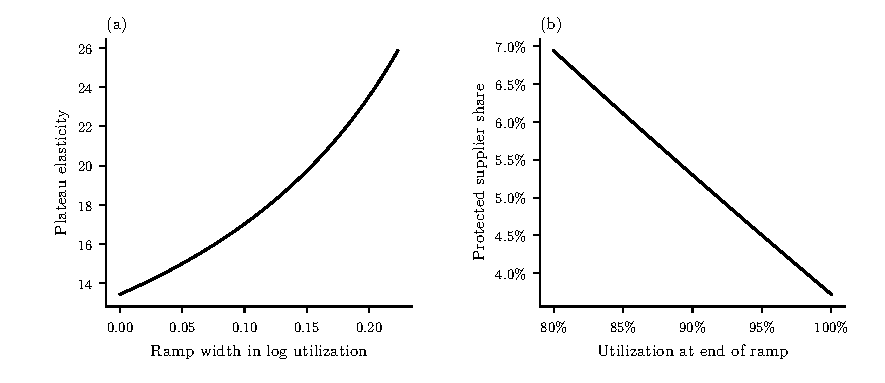
\includegraphics[width=\textwidth]{A04-smoothing-cost.pdf}
\caption{(a) Plateau elasticity against ramp width, with $0\leq w\leq L$. (b) The corresponding protected share against the utilization where the ramp ends. The value $K^*$ is reached only in the nonsmooth limit $w=0$.}
\label{fig:smoothness-cost}
\end{figure}



\clearpage
\section{The Full Supplier Limit}
\label{app:full}

Setting $\alpha=1$ gives $\eta\leq0$. When one supplier owns all deposits, $TU=B$ and their income is $I=BR_b(U)$. Depositing while $B$ remains fixed reduces utilization and therefore income wherever the borrow rate is increasing. Equivalently,
\[
\frac{dI}{d\delta}=-U^2R_b'(U)
\]
No strictly increasing rate curve can protect this supplier. A flat rate gives equality. Figure~\ref{fig:full-supplier-income} uses the single kink example with a $1\%$ floor, a supplier initially holding all \$10 million of supply and \$9.5 million of fixed borrowing. The plotted interval remains on rising portions of the curve; a sufficiently large deposit would eventually reach the flat floor.

\begin{figure}[htbp]
\centering
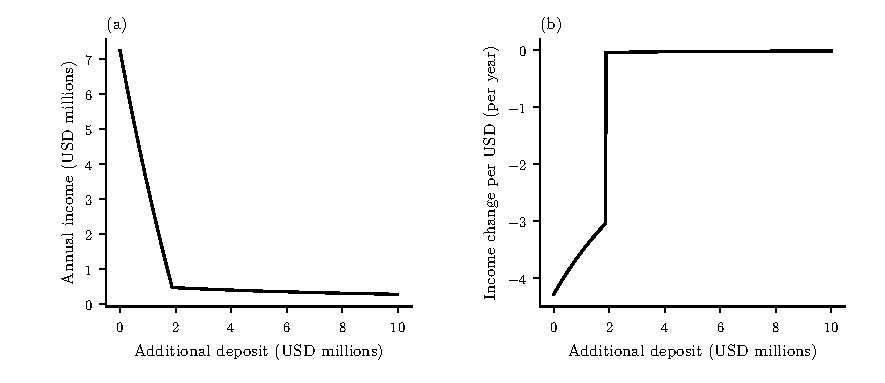
\includegraphics[width=\textwidth]{A01-full-supplier.pdf}
\caption{A supplier owning the whole pool: (a) annualized income and (b) its marginal change under additional deposits. The guarantee cannot hold on a rising rate branch.}
\label{fig:full-supplier-income}
\end{figure}



\end{document}
